\documentclass[11pt]{article}
\usepackage[a4paper,margin=1in]{geometry}
\usepackage{amsmath,amssymb,amsfonts,mathtools}
\usepackage{graphicx}
\usepackage{booktabs}
\usepackage{hyperref}
\usepackage{enumitem}
\setlist[enumerate]{label=(\arabic*),leftmargin=1.8em,itemsep=0.35em,topsep=0.5em}

\hypersetup{colorlinks=true,linkcolor=blue,urlcolor=blue,citecolor=blue}

\title{Project Report for PhD Level Pass (Math 589)\\\large Minimum-Variance Portfolio with Detrended Returns and KKT Solution}
\author{Dimitri Bolt}
\date{\today}

\begin{document}
	\maketitle
	
	\noindent\textbf{Industry supervision:} Morgan Stanley \quad
	\textbf{Academic supervision:} Mikhail Stepanov
	
	\bigskip
	
	\section{Overview and Objectives}
	\begin{itemize}
		\item \textbf{Goal.} Implement and audit the classical Markowitz baseline---minimum variance with a target return---on real equity data; exhibit its numerical fragility; motivate Random Matrix Theory (RMT) covariance cleaning.
		%
		\begin{itemize}
			\item \textit{Context.} Modern Portfolio Theory (MPT) is a framework dating back to Markowitz's foundational work \textit{Portfolio Selection} (1952) and its monograph extension (1959).
It was a serious theoretical breakthrough with a Nobel Prize awarded for it, but practitioners in the field of economics expressed serious doubts about the validity of this approach in practice. Among the objections to this approach are cautions about its practical robustness.
 In particular, small estimation errors in $(\mu,\Sigma)$ can produce unstable and implausible weights (Michaud, 1989); naïve $1/N$ diversification can outperform optimized MPT in realistic settings (DeMiguel, Garlappi \& Uppal, 2009); empirical covariance matrices are noisy in high dimension and benefit from shrinkage (Ledoit \& Wolf, 2004); and Random-Matrix-Theory analyses show that most sample eigenstructure is dominated by noise (Laloux, Cizeau, Bouchaud \& Potters, 1999). 
			 
			\item \textit{Problem statement in this report.} The purpose of this project is to test using real,  observational data on stocks, whether the Markowitz portfolio selection is stable to small perturbations or from day-to-day variations, following the objections raised in the references above.
			\item \textit{Why this matters.} Practitioners (and clients) expect continuity: when market conditions change little from “yesterday” to “today,” the recommended portfolio \(w_t\) should remain close to \(w_{t-1}\). Large, frequent swings undermine practical usability.
			\item \textit{What we test and how.} We deliberately make the benchmark \emph{favorable} to the baseline: choose \(200\) of the most stable, weakly correlated equities (no cherry-picking of ``difficult'' names), vary inputs only by \emph{natural} day-over-day updates of \((\mu,\Sigma)\) (no artificial noise), and measure stability by
			\[
			\tau_t=\frac{\lVert w_t-w_{t-1}\rVert_{l^1}}{\lVert w_{t-1}\rVert_{l^1}}\times 100\%,\qquad
			\kappa=\text{cond}(\cdot).
			\]
			\item \textit{Intended contribution.} The economics literature frequently \emph{states} instability for empirical mean--variance solutions, but {\bf clear \emph{quantitative} demonstrations of the magnitude of day-to-day swings are rare (to be honest I did not find a numerical estimate)}. This report fills that gap with explicit figures and summary statistics on real data, and sets up the subsequent RPCA/RMT-based improvements.
		\end{itemize}
		\item \textbf{Theoretical foundation.} Sections 6.1 and Appendix M of \href{numbook.pdf}{\emph{Advanced Numerical Methods and High-Performance Computing} by Marek Ryszard Rychlik} (pp.~121--123 and pp.~357--360 in the book pagination).
		\item \textbf{Deliverables.}
		\begin{enumerate}
			\item Vectorized Python implementation in \texttt{log\_returns.py} and \texttt{markowitz\_portfolio.py} (\emph{own code, no loops}, only vector/matrix operations).
			\item KKT-based solver with annualization and diagnostics (condition number, spectrum).
			\item Stability analysis across dates; key figures: \texttt{weight\_change\_l1\_norm\_timeseries\_100.png} and \texttt{weight\_change\_l1\_norm\_timeseries.png}.
		\end{enumerate}
	\end{itemize}
	
	\section{Markowitz Baseline as a Linearly Constrained QP}
	\subsection{Problem statement and notation}
	\begin{itemize}
		\item \textbf{Data objects.}
		
		Risk $\coloneq$ portfolio variance:  $Var(w^\top \cdot r_t) = w^\top \Sigma\, w$
		
		Let the number of assets be $n$ and the portfolio weights be $w\in\mathbb{R}^n$ (long--short allowed).
		
		Let $\mu\in\mathbb{R}^n$ be annualized expected returns,
		
		$\Sigma\in\mathbb{R}^{n\times n}$ the annualized covariance,
		
		$\mathbf{1}\in\mathbb{R}^n$ the all-ones budget vector,
		
		and $d\in\mathbb{R}$ the target expected return (annualized, here $d=0.1$).
		\item \textbf{Optimization problem.}
		\begin{equation}\label{eq:markowitz}
			\min_{w\in\mathbb{R}^n}\; w^\top \Sigma\, w
			\quad\text{s.t.}\quad
			\mu^\top w = d,\quad \mathbf{1}^\top w = 1.
		\end{equation}
		\item \textbf{Interpretation of symbols.}
		\begin{itemize}
			\item $w$: portfolio weights; $\sum_i w_i=1$ encodes full-investment budget.
			\item $\Sigma$: covariance of (annualized) returns; positive definite in the ideal case.
			\item $\mu$: vector of (annualized) expected returns.
			\item $d$: target portfolio expected return.
			\item $\mathbf{1}$: budget vector enforcing the sum-to-one constraint.
		\end{itemize}
	\end{itemize}
	
	\subsection{KKT system (Karush--Kuhn--Tucker)}
	\begin{itemize}
		\item \textbf{Lagrangian.} Define $\mathcal{L}(w,\lambda,\nu)=\tfrac12 w^\top \Sigma w-\lambda(\mu^\top w-d)-\nu(\mathbf{1}^\top w-1)$.
		\item \textbf{First-order optimality.}
		\begin{enumerate}
			\item Stationarity: $\nabla_w\mathcal{L}=\Sigma w-\lambda\mu-\nu\mathbf{1}=0$.
			\item Primal feasibility: $\mu^\top w=d$, $\mathbf{1}^\top w=1$.
		\end{enumerate}
		\item \textbf{Linear KKT system.}
		\begin{equation}\label{eq:kkt}
			\begin{bmatrix}
				\Sigma & -\mu & -\mathbf{1} \\
				-\mu^\top & 0 & 0 \\
				-\mathbf{1}^\top & 0 & 0
			\end{bmatrix}
			\begin{bmatrix}
				w \\ \lambda \\ \nu
			\end{bmatrix}
			=
			\begin{bmatrix}
				0 \\ -d \\ -1
			\end{bmatrix},
		\end{equation}
		where the left block is the KKT matrix and the right-hand side (rhs) encodes the constraints.
		\item \textbf{Equivalent sign convention.} 
		
		One may flip the constraint signs to obtain
		$\begin{bmatrix}\Sigma & \mu & \mathbf{1}\\ \mu^\top & 0 & 0\\ \mathbf{1}^\top & 0 & 0\end{bmatrix}
		\begin{bmatrix}w\\ \lambda\\ \nu\end{bmatrix}
		=
		\begin{bmatrix} 0\\ d \\ 1\end{bmatrix}$;
		
		 both yield identical $w$.
	\end{itemize}
	
	\subsection{Closed-form via Schur complement (fully derived)}
	\begin{itemize}
		\item \textbf{Stationarity solution.} From $\Sigma w-\lambda\mu-\nu\mathbf{1}=0$ we get $w=\Sigma^{-1}(\lambda\mu+\nu\mathbf{1})$.
		\item \textbf{Solve for $(\lambda,\nu)$.}
		\begin{enumerate}
			\item Return: $\mu^\top w=\mu^\top\Sigma^{-1}(\lambda\mu+\nu\mathbf{1})=d$.
			\item Budget: $\mathbf{1}^\top w=\mathbf{1}^\top\Sigma^{-1}(\lambda\mu+\nu\mathbf{1})=1$.
		\end{enumerate}
		\item \textbf{Define scalars.} $A=\mathbf{1}^\top\Sigma^{-1}\mathbf{1}$, $B=\mathbf{1}^\top\Sigma^{-1}\mu$, $C=\mu^\top\Sigma^{-1}\mu$, $\Delta=AC-B^2$.
		\item \textbf{2\,$\times$\,2 system.} $\begin{bmatrix}C & B\\ B & A\end{bmatrix}\begin{bmatrix}\lambda\\ \nu\end{bmatrix}=\begin{bmatrix}d\\ 1\end{bmatrix}$ gives $\lambda=\dfrac{A d-B}{\Delta}$, $\nu=\dfrac{C-B d}{\Delta}$.
		\item \textbf{Closed-form weights.}
		\begin{equation}\label{eq:closed-form}
			w(d)=\Sigma^{-1}\Big(\tfrac{A d-B}{\Delta}\,\mu+\tfrac{C-B d}{\Delta}\,\mathbf{1}\Big).
		\end{equation}
		\item \textbf{Reference.} Sec.~6.1 in \href{numbook.pdf}{Rychlik, \emph{Advanced Numerical Methods and High-Performance Computing}} presents Markowitz as a linearly constrained QP and the KKT approach.
	\end{itemize}
	
	\section{Data, Detrending, and Annualization}
	\subsection{Data preparation and daily moments}
	\begin{itemize}
		\item \textbf{Prices to log-returns.} For close prices $p_i(t)$: $r_i(t)=\log p_i(t)-\log p_i(t-1)$.
		\item \textbf{Detrended matrix.} Stack detrended daily log-returns into $R\in\mathbb{R}^{T\times n}$.
		\item \textbf{Daily moments.}\;Means $\hat{\mu}_d=\tfrac1T\sum_{t=1}^T r(t)$ and covariance $\Sigma_d=\operatorname{Cov}(R)$.
	\end{itemize}
	
	\subsection{Proof that $\Sigma_{\text{annualized}}=f\cdot\Sigma_d$ and reconciliation with Appendix M}
	\begin{itemize}
		\item \textbf{Setup.} Let daily log-returns be $X_t\in\mathbb{R}^n$ with $\mathbb{E}[X_t]=\hat{\mu}_d$ and $\operatorname{Cov}(X_t)=\Sigma_d$. For $f$ trading days per year define the annual log-return $S_f=\sum_{t=1}^{f} X_t$.
		\item \textbf{Mean and covariance of sum.} $\mathbb{E}[S_f]=f\,\hat{\mu}_d$; $\operatorname{Cov}(S_f)=\sum_{t=1}^{f}\operatorname{Cov}(X_t)+\sum_{s\neq t}\operatorname{Cov}(X_s,X_t)$.
		\item \textbf{Independence (or negligible cross-covariances).} If $X_t$ are i.i.d., then $\operatorname{Cov}(X_s,X_t)=0$ for $s\neq t$, so $\operatorname{Cov}(S_f)=f\,\Sigma_d$. Thus $\boxed{\Sigma_{\text{annualized}}=f\cdot\Sigma_d}$. For weak dependence one gets $\operatorname{Cov}(S_f)=f\,\Sigma_d+2\sum_{h=1}^{f-1}(f-h)\,\Gamma(h)$ with $\Gamma(h)=\operatorname{Cov}(X_t,X_{t+h})$, and the linear rule is an accurate approximation when $\Gamma(h)$ are small.
		\item \textbf{Reconciliation with Appendix M.} Appendix M discusses annualization conventions. Using \emph{log-returns as sums} gives variance additivity: covariance scales by $f$, while standard deviation scales by $\sqrt{f}$. Deviations arise when mixing levels vs returns or sum vs average.
	\end{itemize}
	
	\newpage
	
	\section{Implementation: Fully Vectorized Pipeline (Own Code)}
	\subsection{What \texttt{log\_returns.py} does}
	\begin{itemize}
		\item Build detrended daily log-returns DataFrame \texttt{detrended\_returns\_df}.
		\item Compute $\hat{\mu}_d$ and $\Sigma_d$ in \emph{vectorized} form (no Python loops).
		\item Persist intermediate outputs for the solver stage.
	\end{itemize}
	
	\subsection{What \texttt{markowitz\_portfolio.py} does}
	\begin{itemize}
		\item Annualize via $\mu=f\cdot\hat{\mu}_d$ and $\Sigma=f\cdot\Sigma_d$.
		\item Solve the KKT system \eqref{eq:kkt} for $(w,\lambda,\nu)$ using \emph{only} dense linear algebra (no loops).
		\item Report scalars and plots: budget check, achieved return $\mu^\top w$, variance $w^\top\Sigma w$, standard deviation, $\kappa(\Sigma)$, and spectrum of $\Sigma$.
		\item \textbf{Efficiency highlight.} The implementation is \emph{my own} and \emph{loop-free}; everything is written in vector/matrix form, which is more efficient than loop-based textbook pseudocode.
	\end{itemize}
	
	\section{Experimental Methodology (Design Choices)}
	\subsection{Universe and \emph{non}-cherry-picking justification}
	\begin{itemize}
		\item Real mutual funds typically hold $1500$--$10000$ assets.
		\item To \emph{ease} the task (not to cherry-pick), we select $200$ of the most stable companies: lowest empirical variance and low pairwise correlations.
		\item This choice \emph{simplifies} the benchmark for Markowitz: even a practitioner could construct a reasonable portfolio manually on such a calm universe; the algorithm is deliberately not stressed by extreme volatility or high correlations.
	\end{itemize}
	
	\subsection{Method for Varying the Input Return Vector $r$ (daily natural variation)}
	\begin{itemize}
		\item We vary the input $r$ \emph{only} by moving forward one trading day: the estimate $\mu$ (hence $r$) and $\Sigma$ are recomputed from the updated daily window.
		\item Between ``yesterday'' and ``today'' the market typically changes little; thus $(\mu,\Sigma)$ shift slightly, so a client reasonably expects $w_t$ to be close to $w_{t-1}$ when targeting the same $d$.
		\item This section explicitly describes the \emph{input variation method}: no artificial noise is injected; $r$ varies by natural time evolution of the data.
	\end{itemize}
	
	\newpage
	
	\section{Results and Diagnostics}
	\subsection{Turnover time series: small-asset sanity check}
	\begin{itemize}
		\item Define the relative $\ell_1$ turnover: $\displaystyle \tau_t=\frac{\|w_t-w_{t-1}\|_{l^1}}{\|w_{t-1}\|_{l^1}}\times 100\%$.
		\item On a \emph{small} universe (a few dozen of the most predictable assets), the portfolio changes are small, as expected by a fund client; see the figure below.
	\end{itemize}
	\begin{center}
		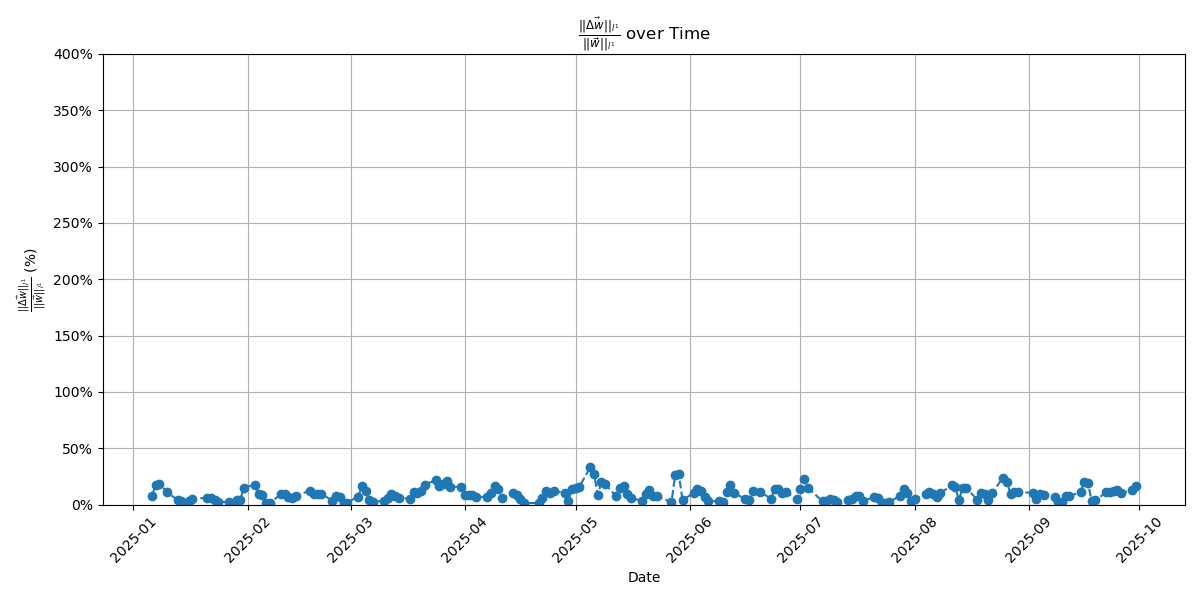
\includegraphics[width=\linewidth]{weight_change_l1_norm_timeseries_100.png}
	\end{center}
	
	% \newpage
	
	\subsection{Conditioning and instability (summary statistics and 200-asset case)}
	\begin{itemize}
		\item However, realistic portfolios contain $1500$--$2000$ assets. Applying Markowitz even to just $200$ assets (still the most stable and predictable) leads to instability: \emph{weights change significantly from day to day.}
		%
		\begin{itemize}
			
			\item \textit{Visual clarification.} The “small-universe” panel shows \emph{single-digit percent} changes (units of percent). The “200-asset” panel naturally extends to the \emph{hundreds of percent} range, signaling much larger swings.
			
			\item \textit{Interpretation for practice.} Under the client’s “yesterday \(\approx\) today” expectation, the small-universe behavior is acceptable; the 200-asset behavior violates that expectation and indicates poor day-to-day stability of the naive baseline.
		\end{itemize}
		\item The following figure illustrates the instability on the $200$-asset universe.
	\end{itemize}
	\begin{center}
		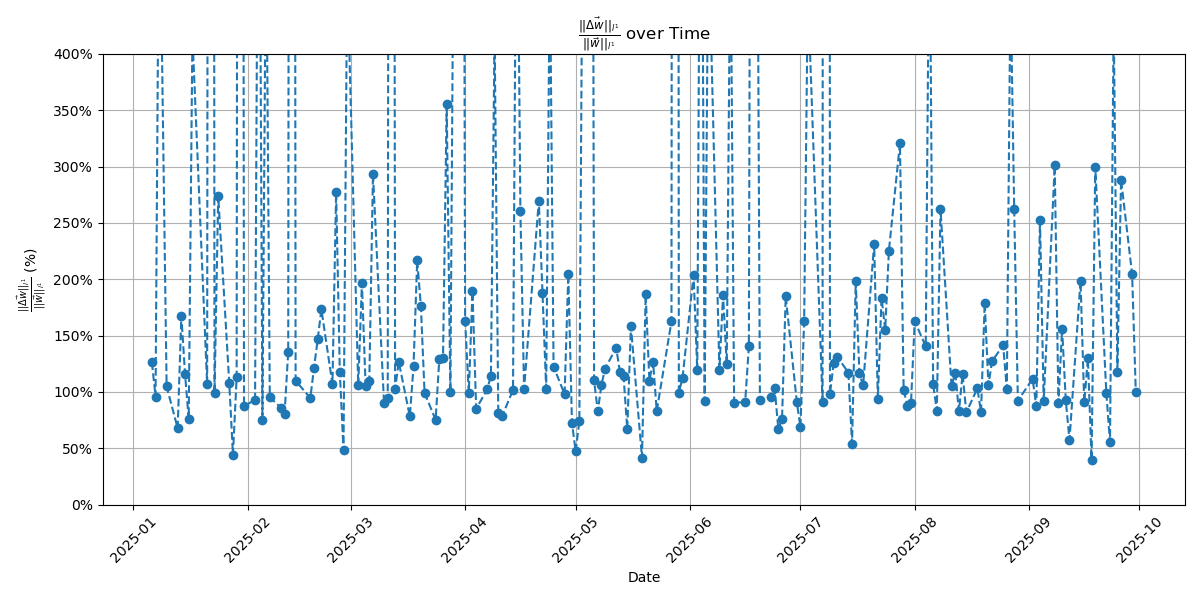
\includegraphics[width=\linewidth]{weight_change_l1_norm_timeseries_200}
	\end{center}
	\begin{itemize}
		\item Summary from \texttt{output\_condition\_numbers.txt} (185 dates):
		\begin{enumerate}
			\item KKT condition number $\kappa$: $\min=4.723\times10^{17}$, $\mathrm{median}=2.161\times10^{18}$, $\mathrm{p}_{75}=4.400\times10^{18}$, $\max=1.664\times10^{22}$.
			\item Relative turnover $\tau_t$: $\mathrm{median}=99\%$, $\mathrm{p}_{75}=140\%$, $\max=18555\%$.
		\end{enumerate}
		\item Interpretation: huge $\kappa$ implies tiny perturbations in $(\mu,\Sigma)$ can cause order-one changes in $w$; observed spikes in $\tau_t$ empirically confirm the instability of the naive baseline even on a friendly universe.
	\end{itemize}
	
	\newpage
	
	\section{Conclusions and Next Steps}
	\subsection{Main conclusions}
	\begin{itemize}
		\item The pure KKT/Markowitz baseline with empirical $\Sigma$ is numerically unstable in practice, producing erratic weights and large turnover.
		\item The root cause is ill-conditioned $\Sigma$ with tiny eigenvalues amplifying estimation noise.
	\end{itemize}
	
	\subsection{Roadmap: RPCA-based Risk Modeling (Course 599) and RMT}
	\begin{itemize}
		\item This study is the initial part of a broader Math~599 project: \emph{RPCA-based Risk Modeling for Portfolio Optimization}. The next stage applies \textbf{Robust PCA (RPCA)} to build a more reliable risk model $\Sigma_{\mathrm{RPCA}}$.
		\item Two natural next steps:
		\begin{enumerate}
			\item Optionally apply \textbf{RMT eigenvalue denoising} to $\Sigma_{\mathrm{RPCA}}$ for extra stability in high-dimensional settings.
			\item Solve the Markowitz problem with realistic constraints and run full backtests: Sharpe, turnover, diversification, risk calibration, and regime-wise stress scenarios.
		\end{enumerate}
	\end{itemize}
	
	\section{References}
	\begin{enumerate}
		\item Marek Ryszard Rychlik, \emph{Advanced Numerical Methods and High-Performance Computing}. Section~6.1 (pp.~121--123) and Appendix~M (pp.~357--360). Local copy: \href{numbook.pdf}{\texttt{numbook.pdf}}.
		\item H. Markowitz (1952), ``Portfolio Selection,'' \emph{The Journal of Finance} 7(1):77--91.
		\item H. Markowitz (1959), \emph{Portfolio Selection: Efficient Diversification of Investments}. John Wiley \& Sons.
		\item R. O. Michaud (1989), ``The Markowitz Optimization Enigma: Is ‘Optimized’ Optimal?,'' \emph{Financial Analysts Journal} 45(1):31--42.
		\item R. Jagannathan and T. Ma (2003), ``Risk Reduction in Large Portfolios: Why Imposing the Wrong Constraints Helps,'' \emph{The Journal of Finance} 58(4):1651--1683.
		\item V. DeMiguel, L. Garlappi, and R. Uppal (2009), ``Optimal versus Naive Diversification: How Inefficient is the 1/N Portfolio Strategy?,'' \emph{The Review of Financial Studies} 22(5):1915--1953.
		\item O. Ledoit and M. Wolf (2004), ``A Well-Conditioned Estimator for Large-Dimensional Covariance Matrices,'' \emph{Journal of Multivariate Analysis} 88(2):365--411.
		\item L. Laloux, P. Cizeau, J.-P. Bouchaud, and M. Potters (1999), ``Noise Dressing of Financial Correlation Matrices,'' \emph{The European Physical Journal B} 6:157--161.
	\end{enumerate}
	
\end{document}
